\documentclass{standalone}
\usepackage{tikz}
\usetikzlibrary{patterns, positioning}


\begin{document}
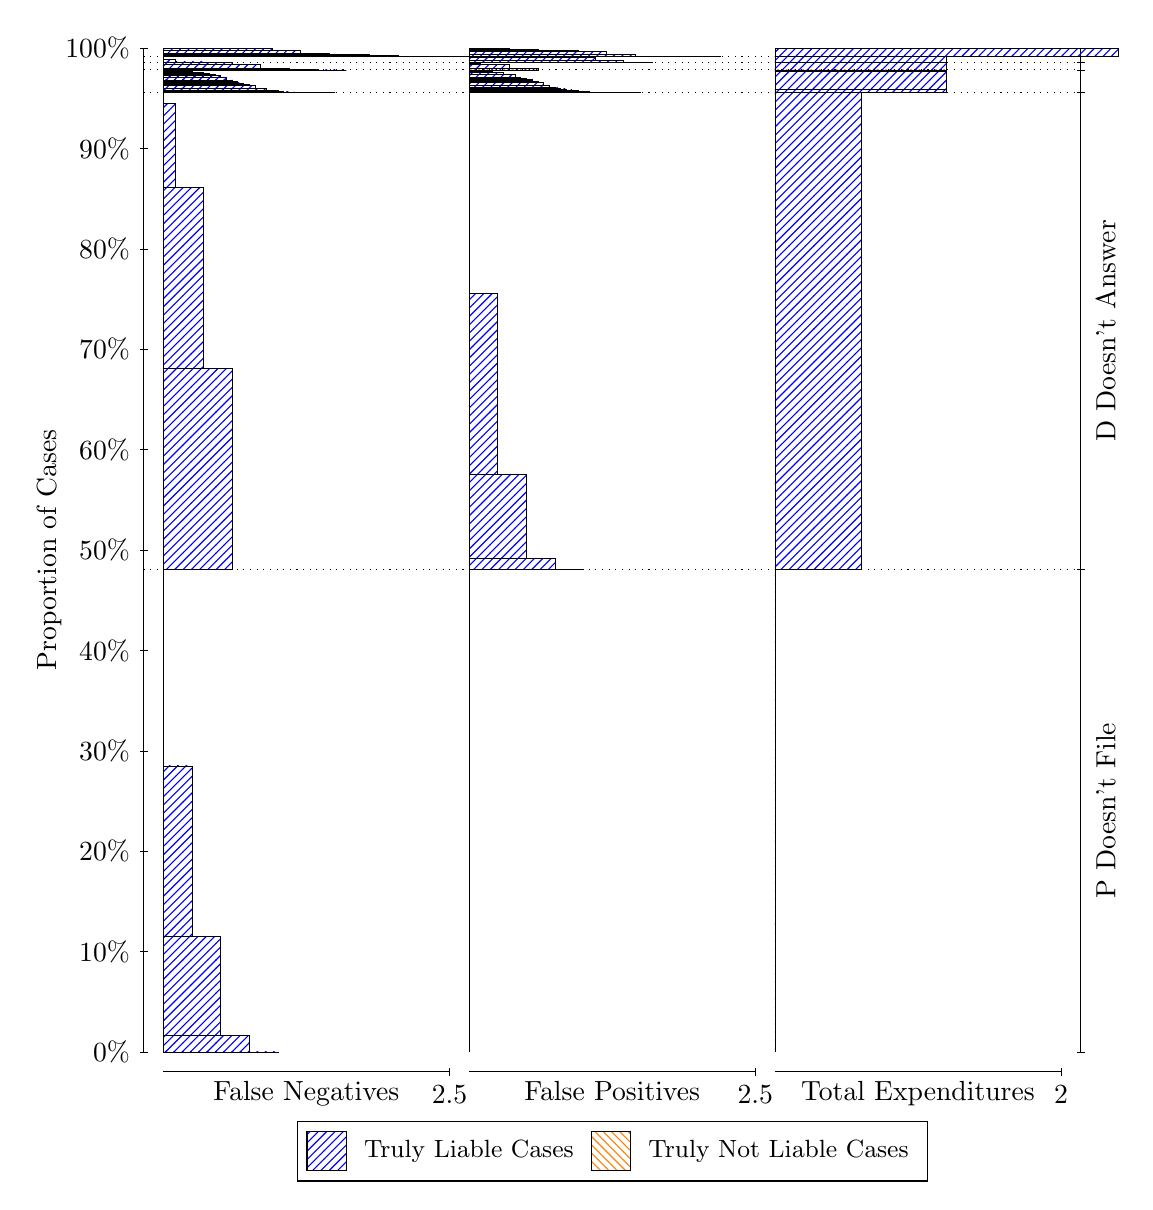
\begin{tikzpicture}
\draw[black, very thin] (1.5,1.75) -- (1.5,14.5);
\node[rotate=90, text=black, anchor=center] at (0.3, 8.125) {Proportion of Cases};
\draw[black, very thin] (1.45,1.75) -- (1.55,1.75);
\node[text=black, anchor=east] at (1.45, 1.75) {0\%};
\draw[black, very thin] (1.45,3.025) -- (1.55,3.025);
\node[text=black, anchor=east] at (1.45, 3.025) {10\%};
\draw[black, very thin] (1.45,4.3) -- (1.55,4.3);
\node[text=black, anchor=east] at (1.45, 4.3) {20\%};
\draw[black, very thin] (1.45,5.575) -- (1.55,5.575);
\node[text=black, anchor=east] at (1.45, 5.575) {30\%};
\draw[black, very thin] (1.45,6.85) -- (1.55,6.85);
\node[text=black, anchor=east] at (1.45, 6.85) {40\%};
\draw[black, very thin] (1.45,8.125) -- (1.55,8.125);
\node[text=black, anchor=east] at (1.45, 8.125) {50\%};
\draw[black, very thin] (1.45,9.4) -- (1.55,9.4);
\node[text=black, anchor=east] at (1.45, 9.4) {60\%};
\draw[black, very thin] (1.45,10.675) -- (1.55,10.675);
\node[text=black, anchor=east] at (1.45, 10.675) {70\%};
\draw[black, very thin] (1.45,11.95) -- (1.55,11.95);
\node[text=black, anchor=east] at (1.45, 11.95) {80\%};
\draw[black, very thin] (1.45,13.225) -- (1.55,13.225);
\node[text=black, anchor=east] at (1.45, 13.225) {90\%};
\draw[black, very thin] (1.45,14.5) -- (1.55,14.5);
\node[text=black, anchor=east] at (1.45, 14.5) {100\%};

\draw[black, very thin] (13.4,1.75) -- (13.4,14.5);
\draw[black, very thin] (13.35,1.75) -- (13.45,1.75);
\node[anchor=west] at (13.35, 1.75) {};
\draw[black, very thin] (13.35,7.8798) -- (13.45,7.8798);
\node[anchor=west] at (13.35, 7.8798) {};
\draw[black, very thin] (13.35,13.933) -- (13.45,13.933);
\node[anchor=west] at (13.35, 13.933) {};
\draw[black, very thin] (13.35,14.223) -- (13.45,14.223);
\node[anchor=west] at (13.35, 14.223) {};
\draw[black, very thin] (13.35,14.313) -- (13.45,14.313);
\node[anchor=west] at (13.35, 14.313) {};
\draw[black, very thin] (13.35,14.389) -- (13.45,14.389);
\node[anchor=west] at (13.35, 14.389) {};
\draw[black, very thin] (13.35,14.5) -- (13.45,14.5);
\node[anchor=west] at (13.35, 14.5) {};

\draw[black, very thin, pattern color=blue, pattern=north east lines] (1.75,1.75) rectangle (3.2033,1.7521);
\draw[black, very thin, pattern color=blue, pattern=north east lines] (1.75,1.7521) rectangle (2.84,1.9626);
\draw[black, very thin, pattern color=blue, pattern=north east lines] (1.75,1.9626) rectangle (2.4767,3.2223);
\draw[black, very thin, pattern color=blue, pattern=north east lines] (1.75,3.2223) rectangle (2.1133,5.3839);
\draw[black, very thin, pattern color=orange, pattern=north west lines] (1.75,5.3839) rectangle (1.75,5.3839);
\draw[black, very thin, pattern color=blue, pattern=north east lines] (1.75,5.3839) rectangle (1.75,7.8798);
\draw[black, very thin, pattern color=blue, pattern=north east lines] (1.75,7.8798) rectangle (2.622,10.427);
\draw[black, very thin, pattern color=blue, pattern=north east lines] (1.75,10.427) rectangle (2.2587,12.729);
\draw[black, very thin, pattern color=blue, pattern=north east lines] (1.75,12.729) rectangle (1.8953,13.793);
\draw[black, very thin, pattern color=orange, pattern=north west lines] (1.75,13.793) rectangle (1.75,13.793);
\draw[black, very thin, pattern color=blue, pattern=north east lines] (1.75,13.793) rectangle (1.75,13.933);
\draw[black, very thin, pattern color=blue, pattern=north east lines] (1.75,13.933) rectangle (3.93,13.933);
\draw[black, very thin, pattern color=blue, pattern=north east lines] (1.75,13.933) rectangle (3.7847,13.933);
\draw[black, very thin, pattern color=blue, pattern=north east lines] (1.75,13.933) rectangle (3.6393,13.933);
\draw[black, very thin, pattern color=blue, pattern=north east lines] (1.75,13.933) rectangle (3.5667,13.935);
\draw[black, very thin, pattern color=blue, pattern=north east lines] (1.75,13.935) rectangle (3.494,13.935);
\draw[black, very thin, pattern color=blue, pattern=north east lines] (1.75,13.935) rectangle (3.4213,13.942);
\draw[black, very thin, pattern color=blue, pattern=north east lines] (1.75,13.942) rectangle (3.3487,13.942);
\draw[black, very thin, pattern color=blue, pattern=north east lines] (1.75,13.942) rectangle (3.276,13.945);
\draw[black, very thin, pattern color=blue, pattern=north east lines] (1.75,13.945) rectangle (3.2033,13.963);
\draw[black, very thin, pattern color=blue, pattern=north east lines] (1.75,13.963) rectangle (3.1307,13.966);
\draw[black, very thin, pattern color=blue, pattern=north east lines] (1.75,13.966) rectangle (3.058,13.966);
\draw[black, very thin, pattern color=blue, pattern=north east lines] (1.75,13.966) rectangle (3.058,13.987);
\draw[black, very thin, pattern color=blue, pattern=north east lines] (1.75,13.987) rectangle (2.9853,13.991);
\draw[black, very thin, pattern color=blue, pattern=north east lines] (1.75,13.991) rectangle (2.9127,14.024);
\draw[black, very thin, pattern color=blue, pattern=north east lines] (1.75,14.024) rectangle (2.9127,14.024);
\draw[black, very thin, pattern color=blue, pattern=north east lines] (1.75,14.024) rectangle (2.84,14.043);
\draw[black, very thin, pattern color=blue, pattern=north east lines] (1.75,14.043) rectangle (2.7673,14.058);
\draw[black, very thin, pattern color=blue, pattern=north east lines] (1.75,14.058) rectangle (2.6947,14.06);
\draw[black, very thin, pattern color=blue, pattern=north east lines] (1.75,14.06) rectangle (2.6947,14.074);
\draw[black, very thin, pattern color=blue, pattern=north east lines] (1.75,14.074) rectangle (2.622,14.094);
\draw[black, very thin, pattern color=blue, pattern=north east lines] (1.75,14.094) rectangle (2.5493,14.133);
\draw[black, very thin, pattern color=blue, pattern=north east lines] (1.75,14.133) rectangle (2.5493,14.134);
\draw[black, very thin, pattern color=blue, pattern=north east lines] (1.75,14.134) rectangle (2.4767,14.152);
\draw[black, very thin, pattern color=blue, pattern=north east lines] (1.75,14.152) rectangle (2.404,14.155);
\draw[black, very thin, pattern color=blue, pattern=north east lines] (1.75,14.155) rectangle (2.404,14.163);
\draw[black, very thin, pattern color=blue, pattern=north east lines] (1.75,14.163) rectangle (2.3313,14.17);
\draw[black, very thin, pattern color=blue, pattern=north east lines] (1.75,14.17) rectangle (2.3313,14.174);
\draw[black, very thin, pattern color=blue, pattern=north east lines] (1.75,14.174) rectangle (2.2587,14.187);
\draw[black, very thin, pattern color=blue, pattern=north east lines] (1.75,14.187) rectangle (2.186,14.195);
\draw[black, very thin, pattern color=blue, pattern=north east lines] (1.75,14.195) rectangle (2.186,14.198);
\draw[black, very thin, pattern color=blue, pattern=north east lines] (1.75,14.198) rectangle (2.1133,14.208);
\draw[black, very thin, pattern color=blue, pattern=north east lines] (1.75,14.208) rectangle (2.0407,14.208);
\draw[black, very thin, pattern color=blue, pattern=north east lines] (1.75,14.208) rectangle (2.0407,14.211);
\draw[black, very thin, pattern color=blue, pattern=north east lines] (1.75,14.211) rectangle (1.968,14.216);
\draw[black, very thin, pattern color=blue, pattern=north east lines] (1.75,14.216) rectangle (1.8953,14.217);
\draw[black, very thin, pattern color=blue, pattern=north east lines] (1.75,14.217) rectangle (1.8227,14.22);
\draw[black, very thin, pattern color=orange, pattern=north west lines] (1.75,14.22) rectangle (1.75,14.22);
\draw[black, very thin, pattern color=blue, pattern=north east lines] (1.75,14.22) rectangle (1.75,14.223);
\draw[black, very thin, pattern color=blue, pattern=north east lines] (1.75,14.223) rectangle (4.0753,14.223);
\draw[black, very thin, pattern color=blue, pattern=north east lines] (1.75,14.223) rectangle (3.712,14.224);
\draw[black, very thin, pattern color=blue, pattern=north east lines] (1.75,14.224) rectangle (3.3487,14.244);
\draw[black, very thin, pattern color=blue, pattern=north east lines] (1.75,14.244) rectangle (2.9853,14.295);
\draw[black, very thin, pattern color=blue, pattern=north east lines] (1.75,14.295) rectangle (2.622,14.313);
\draw[black, very thin, pattern color=orange, pattern=north west lines] (1.75,14.313) rectangle (1.75,14.313);
\draw[black, very thin, pattern color=blue, pattern=north east lines] (1.75,14.313) rectangle (2.622,14.313);
\draw[black, very thin, pattern color=blue, pattern=north east lines] (1.75,14.313) rectangle (2.2587,14.323);
\draw[black, very thin, pattern color=blue, pattern=north east lines] (1.75,14.323) rectangle (1.8953,14.36);
\draw[black, very thin, pattern color=orange, pattern=north west lines] (1.75,14.36) rectangle (1.75,14.36);
\draw[black, very thin, pattern color=blue, pattern=north east lines] (1.75,14.36) rectangle (1.75,14.389);
\draw[black, very thin, pattern color=blue, pattern=north east lines] (1.75,14.389) rectangle (5.8193,14.389);
\draw[black, very thin, pattern color=blue, pattern=north east lines] (1.75,14.389) rectangle (5.456,14.389);
\draw[black, very thin, pattern color=blue, pattern=north east lines] (1.75,14.389) rectangle (5.0927,14.39);
\draw[black, very thin, pattern color=blue, pattern=north east lines] (1.75,14.39) rectangle (4.7293,14.405);
\draw[black, very thin, pattern color=blue, pattern=north east lines] (1.75,14.405) rectangle (4.584,14.405);
\draw[black, very thin, pattern color=blue, pattern=north east lines] (1.75,14.405) rectangle (4.366,14.421);
\draw[black, very thin, pattern color=blue, pattern=north east lines] (1.75,14.421) rectangle (4.2207,14.421);
\draw[black, very thin, pattern color=blue, pattern=north east lines] (1.75,14.421) rectangle (4.0027,14.422);
\draw[black, very thin, pattern color=blue, pattern=north east lines] (1.75,14.422) rectangle (3.8573,14.43);
\draw[black, very thin, pattern color=blue, pattern=north east lines] (1.75,14.43) rectangle (3.6393,14.43);
\draw[black, very thin, pattern color=blue, pattern=north east lines] (1.75,14.43) rectangle (3.494,14.472);
\draw[black, very thin, pattern color=blue, pattern=north east lines] (1.75,14.472) rectangle (3.1307,14.497);
\draw[black, very thin, pattern color=blue, pattern=north east lines] (1.75,14.497) rectangle (2.7673,14.5);
\draw[black, very thin, pattern color=blue, pattern=north east lines] (1.75,14.5) rectangle (2.404,14.5);
\draw[black, very thin, pattern color=blue, pattern=north east lines] (1.75,14.5) rectangle (2.0407,14.5);
\draw[black, very thin, pattern color=orange, pattern=north west lines] (1.75,14.5) rectangle (1.75,14.5);
\draw[black, very thin, pattern color=orange, pattern=north west lines] (5.6333,1.75) rectangle (5.6333,1.75);
\draw[black, very thin, pattern color=blue, pattern=north east lines] (5.6333,1.75) rectangle (5.6333,7.8798);
\draw[black, very thin, pattern color=orange, pattern=north west lines] (5.6333,7.8798) rectangle (7.0867,7.8798);
\draw[black, very thin, pattern color=blue, pattern=north east lines] (5.6333,7.8798) rectangle (7.0867,7.8829);
\draw[black, very thin, pattern color=blue, pattern=north east lines] (5.6333,7.8829) rectangle (6.7233,8.0195);
\draw[black, very thin, pattern color=blue, pattern=north east lines] (5.6333,8.0195) rectangle (6.36,9.083);
\draw[black, very thin, pattern color=blue, pattern=north east lines] (5.6333,9.083) rectangle (5.9967,11.385);
\draw[black, very thin, pattern color=blue, pattern=north east lines] (5.6333,11.385) rectangle (5.6333,13.933);
\draw[black, very thin, pattern color=orange, pattern=north west lines] (5.6333,13.933) rectangle (7.8133,13.933);
\draw[black, very thin, pattern color=blue, pattern=north east lines] (5.6333,13.933) rectangle (7.8133,13.933);
\draw[black, very thin, pattern color=orange, pattern=north west lines] (5.6333,13.933) rectangle (7.668,13.933);
\draw[black, very thin, pattern color=blue, pattern=north east lines] (5.6333,13.933) rectangle (7.668,13.933);
\draw[black, very thin, pattern color=orange, pattern=north west lines] (5.6333,13.933) rectangle (7.5227,13.933);
\draw[black, very thin, pattern color=blue, pattern=north east lines] (5.6333,13.933) rectangle (7.5227,13.933);
\draw[black, very thin, pattern color=blue, pattern=north east lines] (5.6333,13.933) rectangle (7.45,13.936);
\draw[black, very thin, pattern color=orange, pattern=north west lines] (5.6333,13.936) rectangle (7.3773,13.936);
\draw[black, very thin, pattern color=blue, pattern=north east lines] (5.6333,13.936) rectangle (7.3773,13.936);
\draw[black, very thin, pattern color=blue, pattern=north east lines] (5.6333,13.936) rectangle (7.3047,13.939);
\draw[black, very thin, pattern color=orange, pattern=north west lines] (5.6333,13.939) rectangle (7.232,13.939);
\draw[black, very thin, pattern color=blue, pattern=north east lines] (5.6333,13.939) rectangle (7.232,13.939);
\draw[black, very thin, pattern color=blue, pattern=north east lines] (5.6333,13.939) rectangle (7.1593,13.945);
\draw[black, very thin, pattern color=orange, pattern=north west lines] (5.6333,13.945) rectangle (7.0867,13.945);
\draw[black, very thin, pattern color=blue, pattern=north east lines] (5.6333,13.945) rectangle (7.0867,13.948);
\draw[black, very thin, pattern color=blue, pattern=north east lines] (5.6333,13.948) rectangle (7.014,13.958);
\draw[black, very thin, pattern color=orange, pattern=north west lines] (5.6333,13.958) rectangle (6.9413,13.958);
\draw[black, very thin, pattern color=blue, pattern=north east lines] (5.6333,13.958) rectangle (6.9413,13.969);
\draw[black, very thin, pattern color=blue, pattern=north east lines] (5.6333,13.969) rectangle (6.8687,13.982);
\draw[black, very thin, pattern color=orange, pattern=north west lines] (5.6333,13.982) rectangle (6.796,13.982);
\draw[black, very thin, pattern color=blue, pattern=north east lines] (5.6333,13.982) rectangle (6.796,13.985);
\draw[black, very thin, pattern color=blue, pattern=north east lines] (5.6333,13.985) rectangle (6.796,13.993);
\draw[black, very thin, pattern color=blue, pattern=north east lines] (5.6333,13.993) rectangle (6.7233,14.004);
\draw[black, very thin, pattern color=orange, pattern=north west lines] (5.6333,14.004) rectangle (6.6507,14.004);
\draw[black, very thin, pattern color=blue, pattern=north east lines] (5.6333,14.004) rectangle (6.6507,14.022);
\draw[black, very thin, pattern color=blue, pattern=north east lines] (5.6333,14.022) rectangle (6.578,14.062);
\draw[black, very thin, pattern color=blue, pattern=north east lines] (5.6333,14.062) rectangle (6.5053,14.082);
\draw[black, very thin, pattern color=blue, pattern=north east lines] (5.6333,14.082) rectangle (6.4327,14.095);
\draw[black, very thin, pattern color=blue, pattern=north east lines] (5.6333,14.095) rectangle (6.4327,14.098);
\draw[black, very thin, pattern color=blue, pattern=north east lines] (5.6333,14.098) rectangle (6.36,14.113);
\draw[black, very thin, pattern color=blue, pattern=north east lines] (5.6333,14.113) rectangle (6.2873,14.132);
\draw[black, very thin, pattern color=blue, pattern=north east lines] (5.6333,14.132) rectangle (6.2147,14.165);
\draw[black, very thin, pattern color=blue, pattern=north east lines] (5.6333,14.165) rectangle (6.142,14.169);
\draw[black, very thin, pattern color=blue, pattern=north east lines] (5.6333,14.169) rectangle (6.0693,14.19);
\draw[black, very thin, pattern color=blue, pattern=north east lines] (5.6333,14.19) rectangle (6.0693,14.19);
\draw[black, very thin, pattern color=blue, pattern=north east lines] (5.6333,14.19) rectangle (5.9967,14.193);
\draw[black, very thin, pattern color=blue, pattern=north east lines] (5.6333,14.193) rectangle (5.924,14.211);
\draw[black, very thin, pattern color=blue, pattern=north east lines] (5.6333,14.211) rectangle (5.8513,14.214);
\draw[black, very thin, pattern color=blue, pattern=north east lines] (5.6333,14.214) rectangle (5.7787,14.214);
\draw[black, very thin, pattern color=blue, pattern=north east lines] (5.6333,14.214) rectangle (5.706,14.22);
\draw[black, very thin, pattern color=blue, pattern=north east lines] (5.6333,14.22) rectangle (5.6333,14.223);
\draw[black, very thin, pattern color=orange, pattern=north west lines] (5.6333,14.223) rectangle (6.5053,14.223);
\draw[black, very thin, pattern color=blue, pattern=north east lines] (5.6333,14.223) rectangle (6.5053,14.241);
\draw[black, very thin, pattern color=blue, pattern=north east lines] (5.6333,14.241) rectangle (6.142,14.292);
\draw[black, very thin, pattern color=blue, pattern=north east lines] (5.6333,14.292) rectangle (5.7787,14.312);
\draw[black, very thin, pattern color=blue, pattern=north east lines] (5.6333,14.312) rectangle (5.6333,14.313);
\draw[black, very thin, pattern color=orange, pattern=north west lines] (5.6333,14.313) rectangle (7.9587,14.313);
\draw[black, very thin, pattern color=blue, pattern=north east lines] (5.6333,14.313) rectangle (7.9587,14.314);
\draw[black, very thin, pattern color=blue, pattern=north east lines] (5.6333,14.314) rectangle (7.5953,14.342);
\draw[black, very thin, pattern color=blue, pattern=north east lines] (5.6333,14.342) rectangle (7.232,14.38);
\draw[black, very thin, pattern color=blue, pattern=north east lines] (5.6333,14.38) rectangle (6.8687,14.389);
\draw[black, very thin, pattern color=blue, pattern=north east lines] (5.6333,14.389) rectangle (6.5053,14.389);
\draw[black, very thin, pattern color=orange, pattern=north west lines] (5.6333,14.389) rectangle (8.8307,14.389);
\draw[black, very thin, pattern color=blue, pattern=north east lines] (5.6333,14.389) rectangle (8.8307,14.389);
\draw[black, very thin, pattern color=blue, pattern=north east lines] (5.6333,14.389) rectangle (8.4673,14.389);
\draw[black, very thin, pattern color=orange, pattern=north west lines] (5.6333,14.389) rectangle (8.4673,14.389);
\draw[black, very thin, pattern color=blue, pattern=north east lines] (5.6333,14.389) rectangle (8.4673,14.389);
\draw[black, very thin, pattern color=blue, pattern=north east lines] (5.6333,14.389) rectangle (8.104,14.39);
\draw[black, very thin, pattern color=orange, pattern=north west lines] (5.6333,14.39) rectangle (8.104,14.39);
\draw[black, very thin, pattern color=blue, pattern=north east lines] (5.6333,14.39) rectangle (8.104,14.392);
\draw[black, very thin, pattern color=blue, pattern=north east lines] (5.6333,14.392) rectangle (7.7407,14.392);
\draw[black, very thin, pattern color=orange, pattern=north west lines] (5.6333,14.392) rectangle (7.7407,14.392);
\draw[black, very thin, pattern color=blue, pattern=north east lines] (5.6333,14.392) rectangle (7.7407,14.417);
\draw[black, very thin, pattern color=blue, pattern=north east lines] (5.6333,14.417) rectangle (7.3773,14.417);
\draw[black, very thin, pattern color=blue, pattern=north east lines] (5.6333,14.417) rectangle (7.3773,14.459);
\draw[black, very thin, pattern color=orange, pattern=north west lines] (5.6333,14.459) rectangle (7.232,14.459);
\draw[black, very thin, pattern color=blue, pattern=north east lines] (5.6333,14.459) rectangle (7.232,14.459);
\draw[black, very thin, pattern color=blue, pattern=north east lines] (5.6333,14.459) rectangle (7.014,14.467);
\draw[black, very thin, pattern color=blue, pattern=north east lines] (5.6333,14.467) rectangle (6.8687,14.467);
\draw[black, very thin, pattern color=orange, pattern=north west lines] (5.6333,14.467) rectangle (6.8687,14.467);
\draw[black, very thin, pattern color=blue, pattern=north east lines] (5.6333,14.467) rectangle (6.8687,14.469);
\draw[black, very thin, pattern color=blue, pattern=north east lines] (5.6333,14.469) rectangle (6.6507,14.469);
\draw[black, very thin, pattern color=blue, pattern=north east lines] (5.6333,14.469) rectangle (6.5053,14.47);
\draw[black, very thin, pattern color=orange, pattern=north west lines] (5.6333,14.47) rectangle (6.5053,14.47);
\draw[black, very thin, pattern color=blue, pattern=north east lines] (5.6333,14.47) rectangle (6.5053,14.484);
\draw[black, very thin, pattern color=blue, pattern=north east lines] (5.6333,14.484) rectangle (6.2873,14.484);
\draw[black, very thin, pattern color=blue, pattern=north east lines] (5.6333,14.484) rectangle (6.142,14.484);
\draw[black, very thin, pattern color=blue, pattern=north east lines] (5.6333,14.484) rectangle (6.142,14.499);
\draw[black, very thin, pattern color=blue, pattern=north east lines] (5.6333,14.499) rectangle (5.7787,14.499);
\draw[black, very thin, pattern color=blue, pattern=north east lines] (5.6333,14.499) rectangle (5.7787,14.5);
\draw[black, very thin, pattern color=blue, pattern=north east lines] (5.6333,14.5) rectangle (5.6333,14.5);
\draw[black, very thin, pattern color=orange, pattern=north west lines] (9.5167,1.75) rectangle (9.5167,1.75);
\draw[black, very thin, pattern color=blue, pattern=north east lines] (9.5167,1.75) rectangle (9.5167,7.8798);
\draw[black, very thin, pattern color=orange, pattern=north west lines] (9.5167,7.8798) rectangle (10.607,7.8798);
\draw[black, very thin, pattern color=blue, pattern=north east lines] (9.5167,7.8798) rectangle (10.607,13.933);
\draw[black, very thin, pattern color=orange, pattern=north west lines] (9.5167,13.933) rectangle (11.697,13.933);
\draw[black, very thin, pattern color=blue, pattern=north east lines] (9.5167,13.933) rectangle (11.697,13.971);
\draw[black, very thin, pattern color=orange, pattern=north west lines] (9.5167,13.971) rectangle (11.697,13.971);
\draw[black, very thin, pattern color=blue, pattern=north east lines] (9.5167,13.971) rectangle (11.697,14.202);
\draw[black, very thin, pattern color=orange, pattern=north west lines] (9.5167,14.202) rectangle (11.697,14.202);
\draw[black, very thin, pattern color=blue, pattern=north east lines] (9.5167,14.202) rectangle (11.697,14.223);
\draw[black, very thin, pattern color=orange, pattern=north west lines] (9.5167,14.223) rectangle (11.697,14.223);
\draw[black, very thin, pattern color=blue, pattern=north east lines] (9.5167,14.223) rectangle (11.697,14.313);
\draw[black, very thin, pattern color=orange, pattern=north west lines] (9.5167,14.313) rectangle (11.697,14.313);
\draw[black, very thin, pattern color=blue, pattern=north east lines] (9.5167,14.313) rectangle (11.697,14.389);
\draw[black, very thin, pattern color=orange, pattern=north west lines] (9.5167,14.389) rectangle (13.877,14.389);
\draw[black, very thin, pattern color=blue, pattern=north east lines] (9.5167,14.389) rectangle (13.877,14.391);
\draw[black, very thin, pattern color=orange, pattern=north west lines] (9.5167,14.391) rectangle (13.877,14.391);
\draw[black, very thin, pattern color=blue, pattern=north east lines] (9.5167,14.391) rectangle (13.877,14.5);
\draw[black, dotted] (1.5,7.8798) -- (13.4,7.8798);
\draw[black, dotted] (1.5,13.933) -- (13.4,13.933);
\draw[black, dotted] (1.5,14.223) -- (13.4,14.223);
\draw[black, dotted] (1.5,14.313) -- (13.4,14.313);
\draw[black, dotted] (1.5,14.389) -- (13.4,14.389);
\draw[black, very thin] (1.75,1.5) -- (5.3833,1.5);
\node[text=black, anchor=north] at (3.5667, 1.5) {False Negatives};
\draw[black, very thin] (5.3833,1.45) -- (5.3833,1.55);
\node[text=black, anchor=north] at (5.3833, 1.45) {2.5};

\draw[black, very thin] (5.6333,1.5) -- (9.2667,1.5);
\node[text=black, anchor=north] at (7.45, 1.5) {False Positives};
\draw[black, very thin] (9.2667,1.45) -- (9.2667,1.55);
\node[text=black, anchor=north] at (9.2667, 1.45) {2.5};

\draw[black, very thin] (9.5167,1.5) -- (13.15,1.5);
\node[text=black, anchor=north] at (11.333, 1.5) {Total Expenditures};
\draw[black, very thin] (13.15,1.45) -- (13.15,1.55);
\node[text=black, anchor=north] at (13.15, 1.45) {2};

\node[text=black, centered, rotate=90] at (13.72, 4.8149) {P Doesn't File};
\node[text=black, centered, rotate=90] at (13.72, 10.906) {D Doesn't Answer};





\draw (7.449999999999999,1.5) node[draw=none] (baseCoordinate) {};
\begin{scope}[align=center]
        \matrix[scale=0.5, draw=black, below=0.5cm of baseCoordinate, nodes={draw}, column sep=0.1cm]{
            \node[rectangle, draw, minimum width=0.5cm, minimum height=0.5cm, pattern color=blue, pattern=north east lines] {}; &
            \node[draw=none, font=\small, text=black] (B) {Truly Liable Cases}; &
            \node[rectangle, draw, minimum width=0.5cm, minimum height=0.5cm, pattern color=orange, pattern=north west lines] {}; &
            \node[draw=none, font=\small, text=black] (B) {Truly Not Liable Cases}; \\
            };
\end{scope}

\end{tikzpicture}
\end{document}